\section{Results}

\subsection{Main result}
With replanning enabled (R1) the agent passed \MainQ{} of \MainN{} questions (\MainPct\%), using \MainCalls{} model calls in \MainMinutes{} minutes on the GTX 1650, with no timeouts. With replanning disabled (R2) it passed \NoRepQ{} of \NoRepN{} (\NoRepPct\%), using \NoRepCalls{} calls in \NoRepMinutes{} minutes, again with no timeouts. Table~\ref{tab:category} gives the counts by category. The fixed baseline passes all twenty, but several of its answers are assembled by code written for the question outside the tools (Section~IV-C), so it is a ceiling and not a competing result. The twelve scenarios of the recovery suite all passed.

\begin{table}[t]
\caption{Questions passed by category, one run per question. R1: replanning enabled; R2: replanning disabled; Base.\ is the baseline.}
\label{tab:category}
\centering
\footnotesize
\begin{tabular}{lcccc}
\hline
Category & $n$ & R1 & R2 & Base. \\
\hline
filter & 2 & 0 & 0 & 0/6 & 0 & 0/6 & 2 \\
group aggregate & 3 & 3 & 3 & 9/9 & 3 & 9/9 & 3 \\
rank & 3 & 0 & 0 & 0/9 & 0 & 0/9 & 3 \\
period compare & 2 & 2 & 2 & 6/6 & 2 & 6/6 & 2 \\
trend & 2 & 0 & 0 & 0/6 & 0 & 0/6 & 2 \\
contribution & 2 & 2 & 2 & 6/6 & 2 & 6/6 & 2 \\
correlation & 2 & 2 & 2 & 6/6 & 2 & 6/6 & 2 \\
anomalies & 2 & 2 & 2 & 6/6 & 2 & 6/6 & 2 \\
multi-step & 2 & 1 & 1 & 3/6 & 1 & 3/6 & 2 \\
\hline
\textbf{All} & 20 & 12 & 12 & 36/60 & 12 & 36/60 & 20 \\
\hline

\end{tabular}
\end{table}

\subsection{Development history}
The two runs were made after the system had been changed. An earlier version was run once on these same 20 questions. That run showed that the scoring path could not accept several of the answer shapes the tools returned: a ranking by totals needs an aggregation that the ranking tool lacked, a plain total came back as a one-group mapping, a counting question was turned into a mapping by the step that extends filter-only plans (Section~III-C), and the trend direction label followed a rule that differed from the oracle's. We changed the tools and that step accordingly, and the planner model was replaced, before the runs reported here. Because the changes were designed after seeing failures on these questions, the results below are not a held-out measurement. A model-free check that feeds hand-written plans through the same executor, answer extractor and scorer, with a mock model that returns the plan unchanged, finds a passing plan for all \MainReach{} questions on the version evaluated here.

\subsection{Effect of replanning}
Disabling replanning raised the number of questions passed from \MainQ{} to \NoRepQ{}. Eight questions pass only without replanning (q03, q04, q06, q09, q12, q17, q18, q19), none passes only with it, ten pass in both, and q11 and q20 fail in both. For all twenty questions the first plan has the same tool list in both runs, so the difference comes after the first result. In the eight questions the first plan is the one that passes in R2. In R1 the inspection step then returned new tasks, in two to four plan versions, and the agent executed between 3 and 12 tools where R2 executed one or two. The answer handed to the scorer is read from the last executed task, so an added analysis displaced the correct one. For q03 the first plan was a single \texttt{group\_aggregate} of sales by region. Four replanning calls followed, which added \texttt{segment\_contribution}, \texttt{trend}, \texttt{filter}, \texttt{rank} and further tasks, and the final answer was a set of profit shares by segment.

Replanning also cost time: R1 used \MainCalls{} calls and \MainMinutes{} minutes against \NoRepCalls{} calls and \NoRepMinutes{} minutes for R2. This is a measurement of one model with one inspection prompt. It does not show that replanning is harmful in general. The questions need one or two steps, and here the model chose to add analyses when it could have returned an empty list. It does show that a replanning step has to be paired with an answer rule that does not depend on which task ran last.

\subsection{Failures with replanning disabled}
The two failures in R2 are planning failures, and the tools ran correctly in both. For q11 (monthly trend of sales in 2017) the model planned a monthly trend with no restriction to 2017, so the points cover all four years. For q20 (top three cities by sales in the Consumer segment) the model planned a filter, a \texttt{group\_aggregate} by city and a \texttt{rank}, but gave \texttt{rank} no aggregation argument; \texttt{rank} works on the table it is given and not on the grouped output, so it ranked single transactions and returned Seattle, Newark and Detroit.

\subsection{Cost and latency}
Figure~\ref{fig:time} shows where the time went. Almost all of it is spent in the model. In R1, planning took 636 seconds, replanning 971, repair prompts 187, answer synthesis 35, and the tools 3, over the 20 question runs. In R2 there is no replanning time, repair prompts took 9 seconds, and the tools took 1 second. Repair prompts are issued inside planning and replanning calls, so the stage totals overlap and do not add up to the run time.

\begin{figure}[t]
\centering
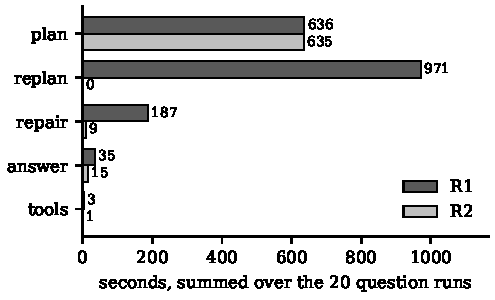
\includegraphics[width=\columnwidth]{figures/fig_stage_time.pdf}
\caption{Seconds spent in each stage, summed over the 20 question runs, with replanning enabled (R1) and disabled (R2). Repair prompts are issued inside the planning and replanning calls, so their time is also counted in those stages.}
\label{fig:time}
\end{figure}

\subsection{Smaller models}
We ran three other local models under the same protocol and the same limits, with replanning enabled. Table~\ref{tab:models} gives the outcome. qwen3:4b-instruct passed \MainQ{} questions, qwen2.5:7b-instruct 8, llama3.2:3b 2 and qwen2.5:3b-instruct 1. No run timed out. ``No answer shape'' counts runs from which the scorer could not build an answer at all; it accounts for 8 of the 12 failures of the 7B model. The 7B model does not fit in 4~GB of GPU memory, so its timings are not comparable. Replanning lowered the score of qwen3:4b-instruct (Section~V-C), so a comparison with replanning enabled understates it, but we did not run the other models with replanning disabled.

\begin{table}[t]
\caption{Four models, one run per question, replanning enabled.}
\label{tab:models}
\centering
\footnotesize
\begin{tabular}{lcccc}
\hline
Model & Passed & Timeouts & No answer shape & Calls \\
\hline
\input{generated/tab_spike_body.tex}
\end{tabular}
\end{table}
